\documentclass[12pt,a4paper]{article}
\usepackage[T1]{fontenc}
\usepackage[utf8]{inputenc}
\usepackage[italian]{babel}
\usepackage{amsmath,amsfonts}
\usepackage{amssymb}
\usepackage{mathtools}
\usepackage{multicol}
\usepackage{array}
\usepackage{pdflscape}
\usepackage[dvipsnames]{xcolor}
\usepackage{colortbl}
\usepackage{graphicx}
\usepackage{wrapfig}	% per didascalie avvolte nel testo
\usepackage{booktabs}
\usepackage{multirow}
\usepackage{parskip}	% pacchetto per la non indentazione del paragrafo
\usepackage{enumitem}	% per elenchi con label
\usepackage{subcaption}	% più performante rispetto subfigure
\usepackage{geometry}	% cambiare la geometria del decumento
\usepackage{tabularx}	% per stabilire autonomamente la larghezza delle tabelle
\usepackage{rotating}   % per ruotare le scritte all'interno delle tabelle
\usepackage{sidecap}	% per le didascalie laterali
\usepackage{longtable}	% per fare tabelle più lunghe di una pagina
\usepackage{eurosym}    % per mettere il simbolo dell'euro
\usepackage{adjustbox}  % per rendere le tabelle più piccole
\usepackage{verbatim}	% per usare l'ambiente comment
\usepackage{pdfpages}	% per includere pdf

% licenza
\usepackage{xmpincl}	% permette di includere licenze in formato XMP
\includexmp{files/CC_Attribution-NonCommercial-ShareAlike_4.0_International}	% file della licenza

% bibliografia
\usepackage[autostyle,italian=guillemets]{csquotes}	% per citare con le virgolette giuste
\usepackage[bibstyle=authoryear,citestyle=authoryear-ibid,backend=biber]{biblatex}	% per la bib
\addbibresource{99-bibliografia.bib}
%\defbibheading{cartaceo}{\section*{Bibliografia cartacea}}
%\defbibheading{web}{\section*{Sitografia}}

% per scrivere bene le unità di misura
\usepackage{siunitx}
\sisetup{
	output-decimal-marker	=	{.},
	list-final-separator	=	{ e },
	list-pair-separator		=	{ e },
	range-phrase			=	{ a },
	per-mode				=	symbol,
    sticky-per 				=	true,
    detect-all				=	true,
}
\DeclareSIUnit\anni{anni}
\DeclareSIUnit\anno{anno}
\DeclareSIUnit\minuti{minuti}
\DeclareSIUnit\minuto{minuto}
\DeclareSIUnit\ore{ore}
\DeclareSIUnit\ora{ora}
\DeclareSIUnit\none{-}
\DeclareSIUnit\e{\euro}

% per personalizzare le caption
\usepackage{caption}
\captionsetup{
	labelformat=simple, % simple senza parentesi, parens con le parentesi
	font={it},
	labelfont=bf,
	justification=centerlast
}

% pacchetto per personalizzare le testatine
\begin{comment}
\usepackage{fancyhdr}
\pagestyle{fancy}
\renewcommand{\chaptermark}[1]{\markboth{#1}{}}
\renewcommand{\sectionmark}[1]{\markright{\thesection\ #1}}
\fancyhf{}
\fancyhead[RO]{\bfseries\rightmark}
\fancyhead[LE]{\bfseries\leftmark}
\fancyfoot[C]{\thepage}
\renewcommand{\headrulewidth}{0.5pt}
\renewcommand{\footrulewidth}{0pt}
\setlength{\headheight}{14pt}
\end{comment}

% serie di pacchetti per la stesura con Latex di grafici e disegni
\usepackage{tikz}
\usepackage{pgfplots}	% pacchetto per grafici
\pgfplotsset{compat=newest}	% ultima versione
\SendSettingsToPgf
\usepgfplotslibrary{fillbetween}	% per riempire di colore i grafici
\usepgfplotslibrary{dateplot}	% per usare date come numeri
\usepgfplotslibrary{statistics}	% per fare boxplot
\usepgfplotslibrary{groupplots}	% per fare grafici a gruppi
\usepgfplotslibrary{external}	% per creare pdf esterni dei grafici
%\tikzexternalize

% per riferimenti
\usepackage{hyperref}
\hypersetup{
	colorlinks	=	true,	% attiva il colore per i link, altrimenti sono inscatolati
	%linkcolor	=	black,	% il colore dei link è nero
	pdftitle	=	Tesi: Dinamiche vegetazionali nel fiume Tagliamento,
	pdfauthor	=	 Castellani Robin,
	%hidelinks,
}

\hyphenation{NDVI}


\begin{document}
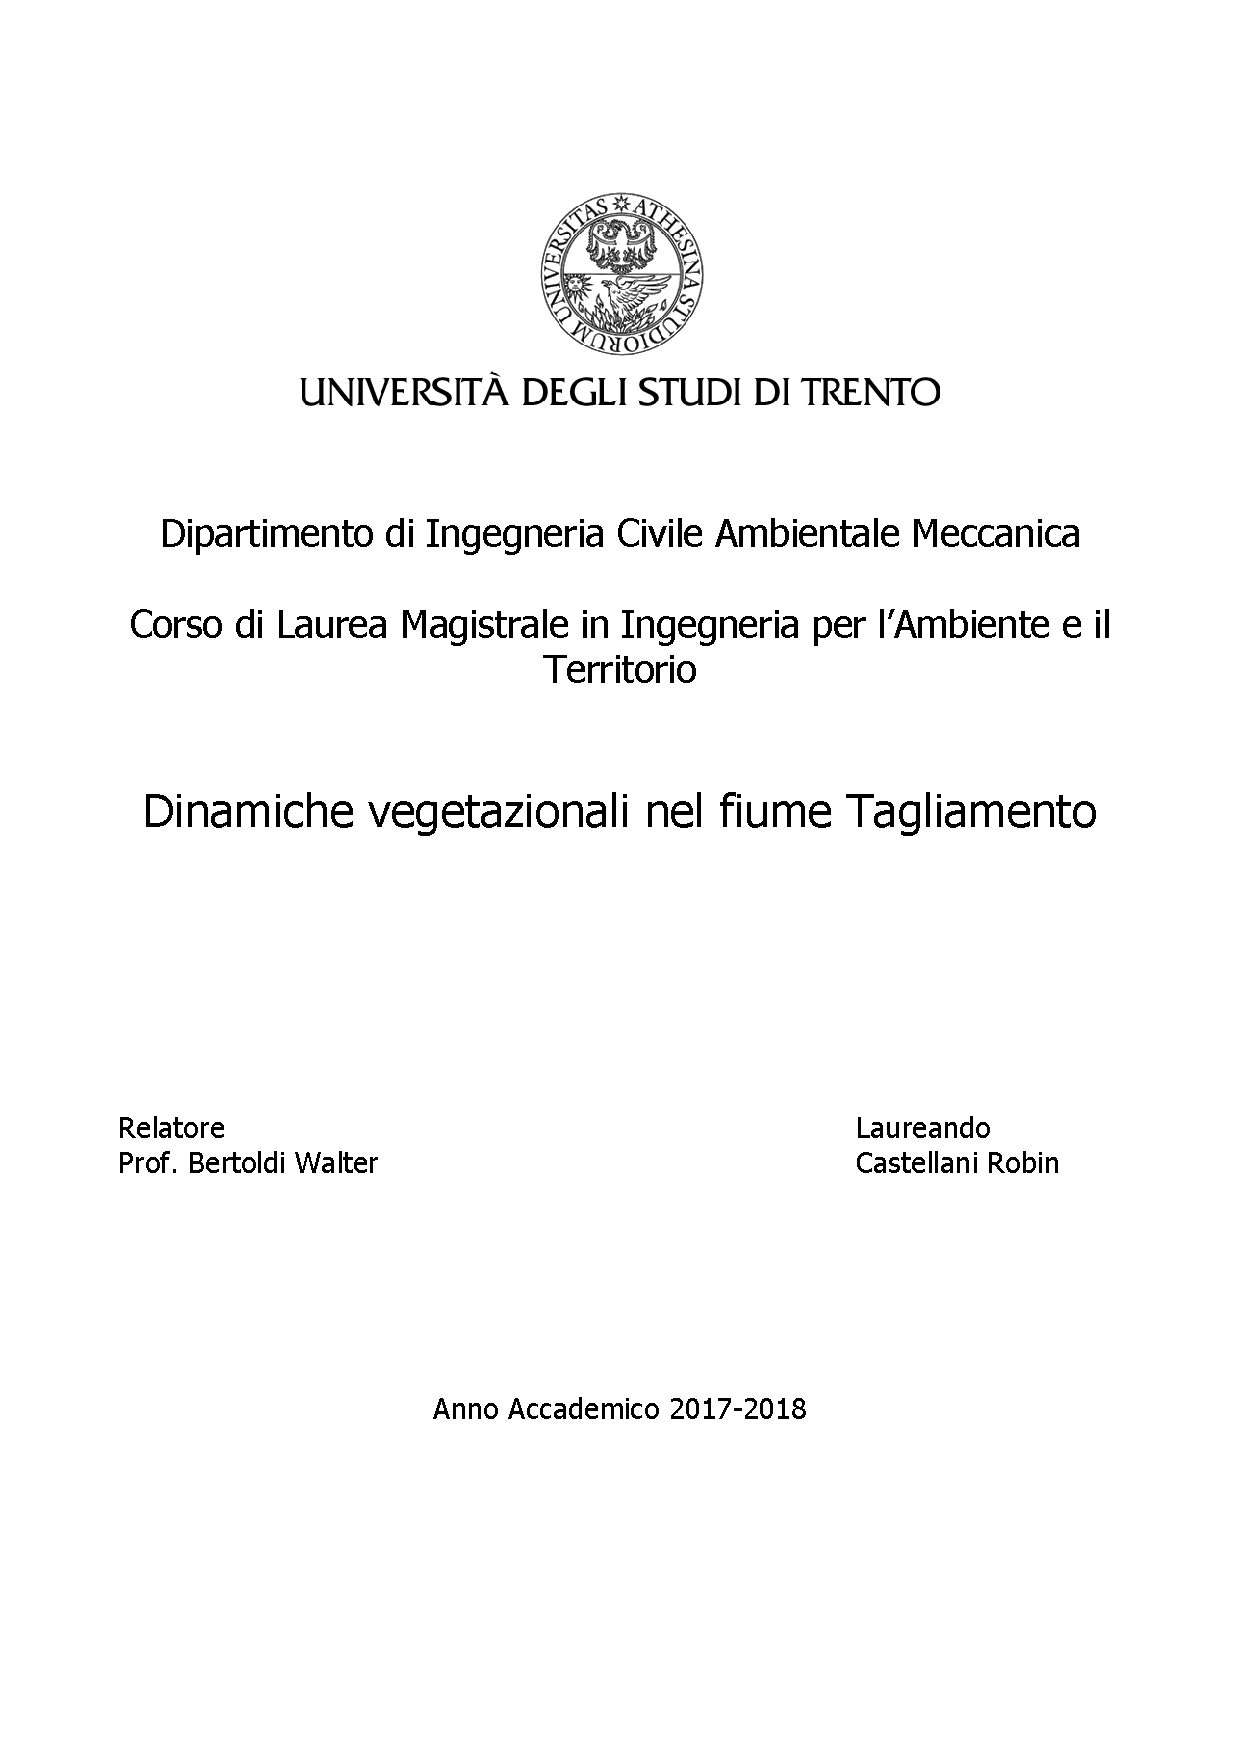
\includepdf[pages=-]{files/frontespizio.pdf}

\pagenumbering{roman}
%----------------------------------------------------------
\begin{abstract}
La presente tesi mira a studiare come cambia la vegetazione nel fiume braided Tagliamento in risposta all'idrologia. 
L'obiettivo principale è quello di ricercare una relazione tra i livelli del pelo libero registrati da alcuni idrometri e la vegetazione erosa, tra i livelli e la quantità di legname che si ritrova in alveo.

Si analizzano immagini satellitari e ortofoto al fine di distinguere la parte vegetata dell'alveo e il legname presente.
Con i dati di piovosità media mensile e di temperatura media mensile si cercano correlazioni con l'espansione della vegetazione che si osserva negli anni.
Dalla quantificazione dell'erosione della vegetazione dovuta alle piene, della quantità di legno in alveo e di un tasso di crescita della vegetazione si tenta di costruire un bilancio di materia vegetale a scala di evento di piena.
Inoltre si trovano valori soglia per l'erosione della vegetazione.
\end{abstract}
%----------------------------------------------------------

\clearpage

\tableofcontents
\listoffigures

\clearpage

\pagenumbering{arabic}

\section{Materiali e metodi}
% materiali
Sono state considerate le bande spettrali del \emph{Near-InfraRed}~(NIR) e del \emph{Red}~(R) nelle immagini satellitari multibande provenienti dalle seguenti missioni:
%
\begin{itemize}
	\item satellite Terra, sensore ASTER Livello~1T (ottenuti in data~21~luglio~2018, \cite{data:ASTER});  
		\\
		NIR (Banda~3N)~\SIrange[range-phrase={-}]{0.78}{0.86}{\nano\m}, R (Banda~2)~\SIrange[range-phrase={-}]{0.63}{0.69}{\micro\m};
	\item costellazione Pleiades (\href{https://pleiades.cnes.fr/en/PLEIADES/index.htm}{Centre National d'Etudes Spatiales}\footnote{\texttt{https://pleiades.cnes.fr/en/PLEIADES/index.htm}}); 
		\\
		NIR~\SIrange[range-phrase={-}]{0.74}{0.94}{\micro\m}, R~\SIrange[range-phrase={-}]{0.59}{0.71}{\micro\m};
	\item satellite Sentinel2A, sensore~MSI Livello~1C (ottenuti in data~21~luglio~2018 tramite la API del \href{http://scihub.copernicus.eu/}{Copernicus Open Access Hub}\footnote{\texttt{http://scihub.copernicus.eu/}});
		\\
		NIR (Banda~8)~\SIrange[range-phrase={-}]{0.763}{0.908}{\micro\m}, R (Banda~4)~\SIrange[range-phrase={-}]{0.645}{0.683}{\micro\m}.
\end{itemize}
%

Le ortofoto dell'estate~2011 provengono dal \href{http://www.pcn.minambiente.it/mattm/}{Portale Cartografico Nazionale del Ministero dell'Ambiente e della tutela del territorio e del mare}\footnote{\texttt{http://www.pcn.minambiente.it/mattm/}};
le ortofoto del~2013 sono state effettuate su commissione; 
%
%
le ortofoto del~2017 sono state ottenute da \href{https://www.google.com/earth/}{Google Earth}\footnote{\texttt{https://www.google.com/earth/}}.
\\
I dati idrometrici sono stati forniti dalla \href{http://www.protezionecivile.fvg.it/it/rete-idrometeorologica}{rete idrometeorologica della Protezione Civile della Regione Autonoma Friuli Venezia Giulia}\footnote{\texttt{http://www.protezionecivile.fvg.it/it/rete-idrometeorologica}}.


% strumenti
\medskip
Per eseguire le analisi sulle immagini aeree e satellitari sono stati utilizzati i GIS GRASS (\cite{soft:GRASS}) e QGIS (\cite{soft:QGIS}). Per il download e il pre-processing delle immagini satellitari è stato usato SCP, plugin di QGIS (\cite{soft:SCP}). Per il download delle ortofoto del~2017 si è utilizzato \href{https://github.com/sourcepole/qgis-openlayers-plugin}{OpenLayers}\footnote{\texttt{https://github.com/sourcepole/qgis-openlayers-plugin}}, plugin di QGIS.


\section{Livelli idrometrici e quantità di vegetazione}
I grafici in figura~\ref{graph:livelli-orto-sat} mostrano rispettivamente i livelli idrometrici registrati presso l'idrometro di Villuzza, corrispondente al ponte di Pinzano, e le date di cui si dispongono ortofoto e immagini satellitari (ASTER, Pleiades, Sentinel2, Google~Earth). 
Nel secondo grafico sono riportati solamente i livelli maggiori di~\SI{2}{\m} in quanto, secondo \cite{Bertoldi:2009-2m}, livelli superiori a tale soglia iniziano ad avere effetti di disturbo sulla vegetazione.
La tabella~\ref{tab:date-orto-sat} mostra le date e la risoluzione delle immagini utilizzate nell'analisi.

\begin{figure}[ht]
	\centering
	\begin{tikzpicture}
	%\begin{groupplot}
	\begin{axis}[
		%name = orto-sat,
		axis y line* = right,
		axis x line* = top,
		%height = .3\textwidth,
		width = \textwidth,
		date coordinates in = x,
		%symbolic y coords = {ASTER,PLEIADES,SENTINEL2,G-EARTH},
		xticklabel = {\year-\month-\day},
		xtick = data,
		ytick = data,
		xticklabel style = {
			rotate = 90,
			anchor = near xticklabel
		},
		enlarge x limits = 0.05,
		enlarge y limits = 0.01,
		ylabel = {Fonte},
		ymax = 3.6,
		ymin = -0.1,
		grid = none,
		only marks,
		]
		\addplot table [x=data, y=numero] {graphics/data/data-orto-sat.txt};
	\end{axis}
	%
	\begin{axis}[
		%name = stages,
		%at = {($(orto-sat.south)-(0,2cm)$)},
		%anchor = north,
		axis y line* = left,
		width = \textwidth,
		date coordinates in = x,
		xticklabel = {\year-\month-\day},
		xticklabel style = {
			rotate = 45,
			anchor = near xticklabel
		},
		enlarge x limits = 0.05,
		enlarge y limits = 0.01,
		ymax = 3.6,
		ymin = -0.1,
		ylabel = {Livello idrometrico},
		grid = major,
		no markers,
		]
		\addplot table [x=data, y=media-gg] {graphics/data/Dati_Villuzza.csv};
	\end{axis}
\end{tikzpicture}
	\tikzsetnextfilename{livelli_2m+imm}
\begin{tikzpicture}
	\begin{axis}[
		width = \textwidth,
		height = 0.5\textwidth,
		date coordinates in = x,
		date ZERO = 2000-01-01,
		xticklabel = {$\year$},
		xticklabel style = {
			rotate = 80,
			anchor = near xticklabel
		},
		xtick distance = 732,
		enlarge x limits = 0.05,
		enlarge y limits = 0.01,
		ymax = 3.7,
		ymin = 1.95,
		ylabel = {Livello idrometrico \si{[\m]}},
		grid = major,
		]
		\addplot+ 
			[red, mark=x, semithick, style=solid, mark=x]
			coordinates {(2000-09-17, 2)(2000-09-17, 3.7)};
		\addplot+ 
			[red, semithick, style=solid, mark=x]
			coordinates {(2001-06-07, 2)(2001-06-07, 3.7)};
		\addplot+
        	[red, semithick, style=solid, mark=x]
        	coordinates {(2002-05-18, 2)(2002-05-18, 3.7)};
		\addplot+
        	[red, semithick, style=solid, mark=x]
        	coordinates {(2002-06-12, 2)(2002-06-12, 3.7)};
		\addplot+
        	[red, semithick, style=solid, mark=x]
        	coordinates {(2003-06-22, 2)(2003-06-22, 3.7)};
		\addplot+
        	[red, semithick, style=solid, mark=x]
        	coordinates {(2004-10-14, 2)(2004-10-14, 3.7)};
		\addplot+
        	[green, semithick, style=solid, mark=x]
        	coordinates {(2005-05-01, 2)(2005-05-01, 3.7)};
		\addplot+
        	[red, semithick, style=solid, mark=x]
        	coordinates {(2005-08-30, 2)(2005-08-30, 3.7)};
		\addplot+
        	[red, semithick, style=solid, mark=x]
        	coordinates {(2006-07-16, 2)(2006-07-16, 3.7)};
		\addplot+
        	[red, semithick, style=solid, mark=x]
        	coordinates {(2007-09-21, 2)(2007-09-21, 3.7)};
		\addplot+
        	[red, semithick, style=solid, mark=x]
        	coordinates {(2008-07-05, 2)(2008-07-05, 3.7)};
		\addplot+
        	[red, semithick, style=solid, mark=x]
        	coordinates {(2009-07-08, 2)(2009-07-08, 3.7)};
		\addplot+
        	[green, semithick, style=solid, mark=x]
        	coordinates {(2010-08-01, 2)(2010-08-01, 3.7)};
		\addplot+
        	[red, semithick, style=solid, mark=x]
        	coordinates {(2010-09-29, 2)(2010-09-29, 3.7)};
		\addplot+
        	[green, semithick, style=solid, mark=x]
        	coordinates {(2011-07-01, 2)(2011-07-01, 3.7)};
		\addplot+
        	[red, semithick, style=solid, mark=x]
        	coordinates {(2012-08-01, 2)(2012-08-01, 3.7)};
		\addplot+
        	[red, semithick, style=solid, mark=x]
        	coordinates {(2013-09-05, 2)(2013-09-05, 3.7)};
		\addplot+
        	[green, semithick, style=solid, mark=x]
        	coordinates {(2013-10-22, 2)(2013-10-22, 3.7)};
		\addplot+
        	[red, semithick, style=solid, mark=x]
        	coordinates {(2014-09-08, 2)(2014-09-08, 3.7)};
		\addplot+
        	[black, semithick, style=solid, mark=x]
        	coordinates {(2014-10-31, 2)(2014-10-31, 3.7)};
       	\addplot+
        	[black, semithick, style=solid, mark=x]
        	coordinates {(2015-08-13, 2)(2015-08-13, 3.7)};
		\addplot+
        	[cyan, semithick, style=solid, mark=x]
        	coordinates {(2015-09-12, 2)(2015-09-12, 3.7)};
		\addplot+
        	[cyan, semithick, style=solid, mark=x]
        	coordinates {(2015-10-22, 2)(2015-10-22, 3.7)};
		\addplot+
        	[cyan, semithick, style=solid, mark=x]
        	coordinates {(2016-09-13, 2)(2016-09-13, 3.7)};
		\addplot+
        	[cyan, semithick, style=solid, mark=x]
        	coordinates {(2017-04-21, 2)(2017-04-21, 3.7)};
		\addplot+
        	[cyan, semithick, style=solid, mark=x]
        	coordinates {(2017-06-13, 2)(2017-06-13, 3.7)};
		\addplot+
        	[green, semithick, style=solid, mark=x]
        	coordinates {(2017-07-07, 2)(2017-07-07, 3.7)};
       	\addplot+
        	[violet, semithick, style=solid, mark=x]
        	coordinates {(2018-06-15, 2)(2018-06-15, 3.7)};
		\addplot+
        	[cyan, semithick, style=solid, mark=x]
        	coordinates {(2018-09-16, 2)(2018-09-16, 3.7)};
		\addplot+
        	[blue, solid, no markers]
        	table [x=data, y=media-gg] {graphics/data/Dati_Villuzza.csv};
	\end{axis}
\end{tikzpicture}
	\caption[livelli idrometrici e foto aeree - satellitari]{in alto il livello idrometrico (in blu) presso l'idrometro di Villuzza. 
	In basso un ingrandimento per i livelli superiori a~\SI{2}{\m}. Le linee indicano le immagini satellitari e le ortofoto considerate (ASTER in magenta, ortofoto in arancione, Pleiades in verde~acqua, Sentinel2 in azzurro, G-Earth in verde).}
	\label{graph:livelli-orto-sat}
\end{figure}




\begin{table}[ht]
	\centering
	\begin{tabular}{c c S[table-format=2.1]}
		\toprule
		Data		&	Fonte		&	\multicolumn{1}{c}{Ris \si{[\m]}}	\\
		\midrule	
		2000-09-17		&	ASTER		&	15	\\
		2001-06-07		&	ASTER		&	15	\\
		2001-12-09		&	ASTER		&	15	\\
		2002-05-18		&	ASTER		&	15	\\
		2002-06-12		&	ASTER		&	15	\\
		2003-06-22		&	ASTER		&	15	\\
		2003-11-29		&	ASTER		&	15	\\
		2004-10-14		&	ASTER		&	15	\\
		2005-08-30		&	ASTER		&	15	\\
		2006-07-16		&	ASTER		&	15	\\
		2007-09-21		&	ASTER		&	15	\\
		2008-07-05		&	ASTER		&	15	\\
		2009-07-08		&	ASTER		&	15	\\
		2010-09-29		&	ASTER		&	15	\\
		2011-06-26/07-02	&	Ortofoto	&	1	\\
		2012-08-01		&	ASTER		&	15	\\
		2013-09-05		&	ASTER		&	15	\\
		2013-10-22		&	Ortofoto	&	0.2	\\
		2014-09-08		&	ASTER		&	15	\\
		2014-10-31		&	Pleiades	\&	0.5	\\
		2015-09-11		&	ASTER		&	15	\\
		2015-09-29		&	Sentinel2	&	10	\\
		2016-09-13		&	Sentinel2	&	10	\\
		2017-04-21		&	Sentinel2	&	10	\\
		2017-06-26/08-02	&	G-Earth	&	0.45	\\
		\bottomrule
	\end{tabular}
	\caption{data e risoluzione delle immagini satellitari e delle ortofoto utilizzate.}
	\label{tab:date-orto-sat}
\end{table}



Si è misurata l'area della vegetazione presente in alveo e nella parte di floodplain soggetta a a forti disturbi (erosione e distacco di isole); 
a tal fine si è seguito l'approccio di altri autori in analisi simili eseguite su immagini ASTER e LandSat~TM \parencites{Bertoldi:2011-ASTER}{Henshaw:2013-LandSat}.
%
\begin{enumerate}
	\item Dapprima è stata individuata manualmente una maschera di calcolo che comprendesse l'alveo attivo e la parte di piana alluvionale che è stata erosa quando coinvolta nelle piene; 
	tale maschera si estende da Tolmezzo al ponte di Madrisio
	(figura~\ref{fig:esempio-maschera}). 
	Applicandola, il dominio computazionale è stato ridotto a comprendere l'inviluppo degli alvei attivi che si sono succeduti dall'immagine del~2000 all'ortofoto del~2017.
	%
	\begin{figure}[ht]
		\centering
		\begin{subfigure}[b]{0.296\textwidth}
			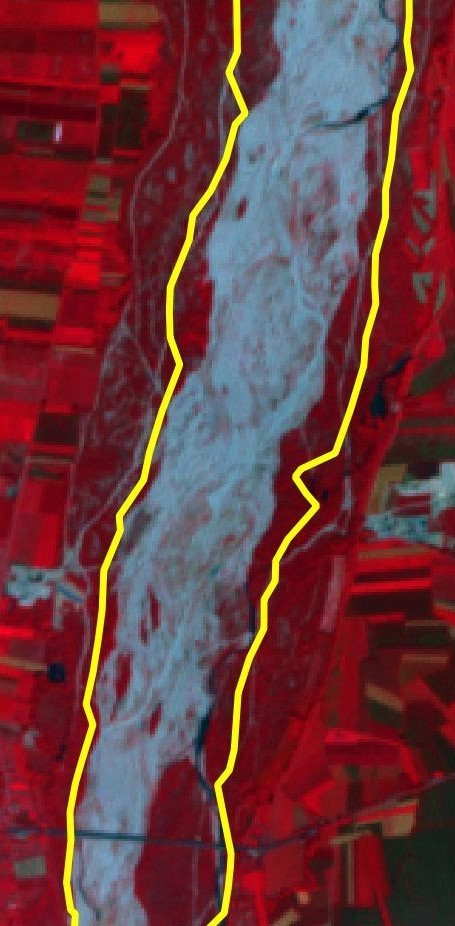
\includegraphics[width=\textwidth]{files/esempio_mask_2000_09_17.jpeg}
			\caption{ASTER 2000-09-17.}
		\end{subfigure}
		\qquad
		\begin{subfigure}[b]{0.30\textwidth}
			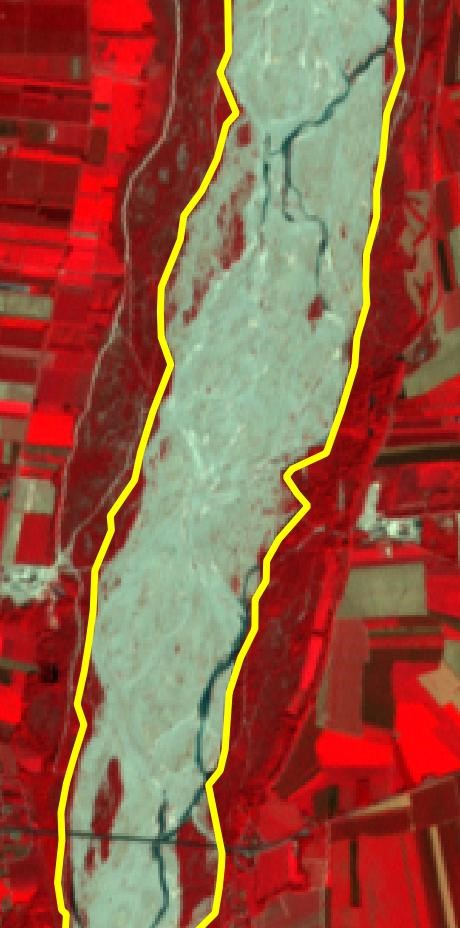
\includegraphics[width=\textwidth]{files/esempio_mask_2015_09_11.jpeg}
			\caption{ASTER 2015-09-11.}
		\end{subfigure}
		\caption[definizione della maschera per limitare il dominio computazionale]
			{esempio in cui si vede come la maschera utilizzata per limitare il dominio computazionale (in giallo) sia il risultato dell'inviluppo degli alvei attivi che si sono modificati nel tempo; le immagini sono in falsi colori (IR-R-G).}
		\label{fig:esempio-maschera}
	\end{figure}
	%
	\item In questa area si è calcolato il \emph{Normalized Difference Vegetation Index} (NDVI) grazie alle bande del \emph{Near Infrared} (NIR) e del \emph{Red} (R)
	%
	\begin{equation}
		%\notag
		NDVI = \frac{NIR - R}{NIR + R} \quad ;
		\label{eq:ndvi}
	\end{equation}
	%
	\item \`{E} stata effettuata una digitalizzazione manuale di alcune aree campione per le immagini ASTER del~2005-08-30 ($\sim 70$) e del~2012-08-01 ($\sim 100$), l'immagine Plaiades del~2014-10-31 ($\sim 40$) e l'immagine Sentinel2 del~2017-04-21 ($\sim 45$) (figura...
	%
	%
	.
	Sono state selezionate immagini per ogni satellite poiché ciascuno è sensibile a bande leggermente diverse; si sono osservate due immagini ASTER dato il grande numero di immagini disponibili scegliendo quelle con minor nuvolosità.
	\item Queste aree campione sono state suddivise in tre classi: vegetazione, alveo attivo e canale.
	Per ogni immagine si è osservata la distribuzione dell'NDVI in ogni classe (figura~\ref{graph:percentili}).
	% 
	\begin{figure}[ht]
		\centering
		\begin{tikzpicture}
	\begin{groupplot}[
		group style = {
			group size = 2 by 3,
			ylabels at = edge left,
			x descriptions at = edge bottom,
			horizontal sep = 1.1cm,
			vertical sep = 0.1cm,
		},
		width = 0.45\textwidth,
		height = 0.45\textwidth,
		ylabel = NDVI,
		boxplot/draw direction = y,
		xtick = {1,2,3},
		xticklabels = {Veg., Alveo, Canale},
		ymax = 0.795,
		ymin = -0.50,
		grid = major,
	]
	\nextgroupplot % ASTER 2005-08-31
		\addplot+ [ % vegetazione
			teal, very thick,
			boxplot prepared = {
				lower whisker = 0.353656,
				lower quartile = 0.470411,
				median = 0.560063,
				upper quartile = 0.614701,
				upper whisker = 0.644957,
				},
        	]
        	coordinates {};
		\addplot+ [ % alveo attivo
			brown, very thick,
			boxplot prepared = {
				lower whisker = 0.077472,
				lower quartile = 0.091653,
				median = 0.122488,
				upper quartile = 0.149573,
				upper whisker = 0.171459,
				},
        	]
        	coordinates {};
		\addplot+ [ % canale
			cyan, very thick,
			boxplot prepared = {
				lower whisker = -0.477885,
				lower quartile = -0.362798,
				median = -0.269905,
				upper quartile = -0.058787,
				upper whisker = 0.072414,
				},
        	]
        	coordinates {};
        \node [fill = white, draw = black, anchor = north east] 
        	at (axis description cs: 1,1) {AST 2005-08-31};
	%------------------------------------------------------
	\nextgroupplot % ASTER 2012-08-01
		\addplot+ [ % vegetazione
			teal, very thick,
			boxplot prepared = {
				lower whisker = 0.341613,
				lower quartile = 0.444200,
				median = 0.586294,
				upper quartile = 0.672889,
				upper whisker = 0.709027,
				},
        	]
        	coordinates {};
		\addplot+ [ % alveo attivo
			brown, very thick,
			boxplot prepared = {
				lower whisker = 0.10506,
				lower quartile = 0.117969,
				median = 0.143631,
				upper quartile = 0.16549,
				upper whisker = 0.184871,
				},
        	]
        	coordinates {};
		\addplot+ [ % canale
			cyan, very thick,
			boxplot prepared = {
				lower whisker = -0.432201,
				lower quartile = -0.379825,
				median = -0.322239,
				upper quartile = -0.226459,
				upper whisker = -0.103914,
				},
        	]
        	coordinates {};
        \node [fill = white, draw = black, anchor = north east] 
        	at (axis description cs: 1,1) {AST 2012-08-01};
	%------------------------------------------------------
	\nextgroupplot % Pleiades 2014-10-31
		\addplot+ [ % vegetazione
			teal, very thick,
			boxplot prepared = {
				lower whisker = 0.286467,
				lower quartile = 0.350238,
				median = 0.415502,
				upper quartile = 0.483495,
				upper whisker = 0.549505,
				},
        	]
        	coordinates {};
		\addplot+ [ % alveo attivo
			brown, very thick,
			boxplot prepared = {
				lower whisker = 0.049796,
				lower quartile = 0.055794,
				median = 0.063049,
				upper quartile = 0.07173,
				upper whisker = 0.081427,
				},
        	]
        	coordinates {};
		\addplot+ [ % canale
			cyan, very thick,
			boxplot prepared = {
				lower whisker = -0.426415,
				lower quartile = -0.387978,
				median = -0.338308,
				upper quartile = -0.266515,
				upper whisker = -0.175373,
				},
        	]
        	coordinates {};
        \node [fill = white, draw = black, anchor = north east] 
        	at (axis description cs: 1,1) {PL 2014-10-31};
	%------------------------------------------------------
	\nextgroupplot % Pleiades 2015-08-13
		\addplot+ [ % vegetazione
			teal, very thick,
			boxplot prepared = {
				lower whisker = 0.415693,
				lower quartile = 0.5,
				median = 0.570359,
				upper quartile = 0.638507,
				upper whisker = 0.704044		
,
				},
        	]
        	coordinates {};
		\addplot+ [ % alveo attivo
			brown, very thick,
			boxplot prepared = {
				lower whisker = 0.075052,
				lower quartile = 0.080858,
				median = 0.087921,
				upper quartile = 0.096031,
				upper whisker = 0.106198,
				},
        	]
        	coordinates {};
		\addplot+ [ % canale
			cyan, very thick,
			boxplot prepared = {
				lower whisker = -0.262599,
				lower quartile = -0.244228,
				median = -0.214393,
				upper quartile = -0.176471,
				upper whisker = -0.132762,
				},
        	]
        	coordinates {};
        \node [fill = white, draw = black, anchor = north east] 
        	at (axis description cs: 1,1) {PL 2015-08-13};
	%------------------------------------------------------
	\nextgroupplot % Sentinel2 2017-04-21
		\addplot+ [ % vegetazione
			teal, very thick,
			boxplot prepared = {
				lower whisker = 0.163722,
				lower quartile = 0.241916,
				median = 0.374344,
				upper quartile = 0.548241,
				upper whisker = 0.672782,
				},
        	]
        	coordinates {};
		\addplot+ [ % alveo attivo
			brown, very thick,
			boxplot prepared = {
				lower whisker = 0.056176,
				lower quartile = 0.061278,
				median = 0.067681,
				upper quartile = 0.076396,
				upper whisker = 0.089304,
				},
        	]
        	coordinates {};
		\addplot+ [ % canale
			cyan, very thick,
			boxplot prepared = {
				lower whisker = -0.322237,
				lower quartile = -0.288822,
				median = -0.239533,
				upper quartile = -0.177094,
				upper whisker = -0.131119,
				},
        	]
        	coordinates {};
        \node [fill = white, draw = black, anchor = north east] 
        	at (axis description cs: 1,1) {S2 2017-04-21};
	%------------------------------------------------------
	\nextgroupplot % WorldView2 2018-06-15
		\addplot+ [ % vegetazione
			teal, very thick,
			boxplot prepared = {
				lower whisker = 0.569665,
				lower quartile = 0.657917,
				median = 0.719523,
				upper quartile = 0.759148,
				upper whisker = 0.791594,
				},
        	]
        	coordinates {};
		\addplot+ [ % alveo attivo
			brown, very thick,
			boxplot prepared = {
				lower whisker = 0.126214,
				lower quartile = 0.129661,
				median = 0.13373,
				upper quartile = 0.138542,
				upper whisker = 0.149326,
				},
        	]
        	coordinates {};
		\addplot+ [ % canale
			cyan, very thick,
			boxplot prepared = {
				lower whisker = -0.416974,
				lower quartile = -0.392405,
				median = -0.365385,
				upper quartile = -0.335135,
				upper whisker = -0.29979,
				},
        	]
        	coordinates {};
        \node [fill = white, draw = black, anchor = north east] 
        	at (axis description cs: 1,1) {WV2 2018-06-15};
	\end{groupplot}
\end{tikzpicture}

		\caption[boxplot dell'NDVI in aree campione in alcune immagini satellitari]{boxplot dell'NDVI in aree campione (diverse decine per ogni immagine) in alcune immagini satellitari.}
		\label{graph:percentili}
	\end{figure}
	%
	\item Da tali grafici sono state ottenute delle soglie di NDVI per classificare le immagini satellitari (tabella~\ref{tab:ndvi-soglia}). Le soglie sono in accordo con quanto riportato in letteratura \parencite{Bertoldi:2011-ASTER}.
	%
	\begin{table}[ht]
		\centering
		\begin{tabular}{
			c 
			S[table-format=1.1]@{\,}
			c@{\,}
			c@{\,}
			c@{\,}
			S[table-format=1.1]
			}
			\toprule
			\multicolumn{6}{c}{\textbf{Soglie}}	\\
			\midrule
			Vegetazione		&	0.2	&	$\leq$	&	NDVI	&		& 	\\
			Alveo attivo	&	0.0	&	$\leq$	&	NDVI	&	$<$		&	0.2	\\
			Canale			&		&			&	NDVI	&	$<$		&	0.0	\\
			\bottomrule
		\end{tabular}
		\caption[soglie NDVI]{soglie di NDVI per la classificazione delle immagini satellitari.}
		\label{tab:ndvi-soglia}
	\end{table}
\end{enumerate}


\begin{figure}[ht]
	\centering
	\begin{tikzpicture}
	\begin{axis}[
		width = \textwidth,
		height = 0.5\textwidth,
		date coordinates in = x,
		date ZERO = 2000-01-01,
		xticklabel = {\year},
		xticklabel style = {
			rotate = 80,
			anchor = near xticklabel
		},
		axis y line* = right,
		ymax = 70,
		%ymin = 0,
		ylabel = {Percentuale di vegetazione},
		grid = none,
		]
		\addplot+
        	[red, mark=+, ultra thick]
        	table [x=data, y=veg] {graphics/data/Class_sat_veg-H2O-ghiaia.txt};
	\end{axis}
	
	\begin{axis}[
		width = \textwidth,
		height = 0.5\textwidth,
		date coordinates in = x,
		date ZERO = 2000-01-01,
		xticklabel = {\year},
		xticklabel style = {
			rotate = 80,
			anchor = near xticklabel
		},
		axis y line* = left,
		axis x line = none,
		enlarge x limits = 0.05,
		enlarge y limits = 0.01,
		ymax = 3.7,
		ymin = 2,
		ylabel = {Livello idrometrico},
		grid = none,
		]
		\addplot+
        	[blue, no markers, ultra thin]
        	table [x=data, y=media-gg] {graphics/data/Dati_Villuzza.csv};
	\end{axis}
\end{tikzpicture}

	\caption[andamento dell'areale della vegetazione nelle isole  e nella floodplain]{andamento dell'areale della vegetazione nelle isole e nella floodplain (in rosso). I dati provengono dalla classificazione delle immagini satellitari (ASTER, Pleiades e Sentinel2). In blu sono mostrati i livelli idrometrici superiori a~\SI{2}{\m} registrati alla stazione di Villuzza.}
	\label{graph:class-sat-veg}
\end{figure}


\clearpage



\printbibliography

\end{document}
